\chapter{Results}
\noindent
\section{Computational Results}

The integration of COMSOL simulations with machine learning resulted in a comprehensive dataset representing various real-world scenarios. The CNN was trained with this data, showing promising accuracy in distinguishing between lead and copper based on the recorded acceleration readings.


\begin{table}[h]
\centering
\begin{tabular}{|r|r|}
  Description & Point graph\\
  X & Height\\
  0 & 5.817362260551916E-20\\
  1 & 5.817362260551916E-20\\
  2 & 6.046114033737459E-20\\
  3 & 5.076492751732623E-20\\
  4 & 2.0101101950650483E-20\\
  5 & 6.082783728329581E-20\\
  6 & 6.082783728329581E-20\\
  7 & 6.082783728329579E-20\\
  8 & 1.3190892577783899E-20\\
  9 & 4.7556868646350063E-20\\
  10 & 4.755686864635008E-20\\
  11 & 4.7556868646350033E-20\\
\end{tabular}

\caption{Result of Lead and Copper after Sinusoidal load has been applied.}
\label{tab:result}
\end{table}



\begin{figure}[t]
  \centering
  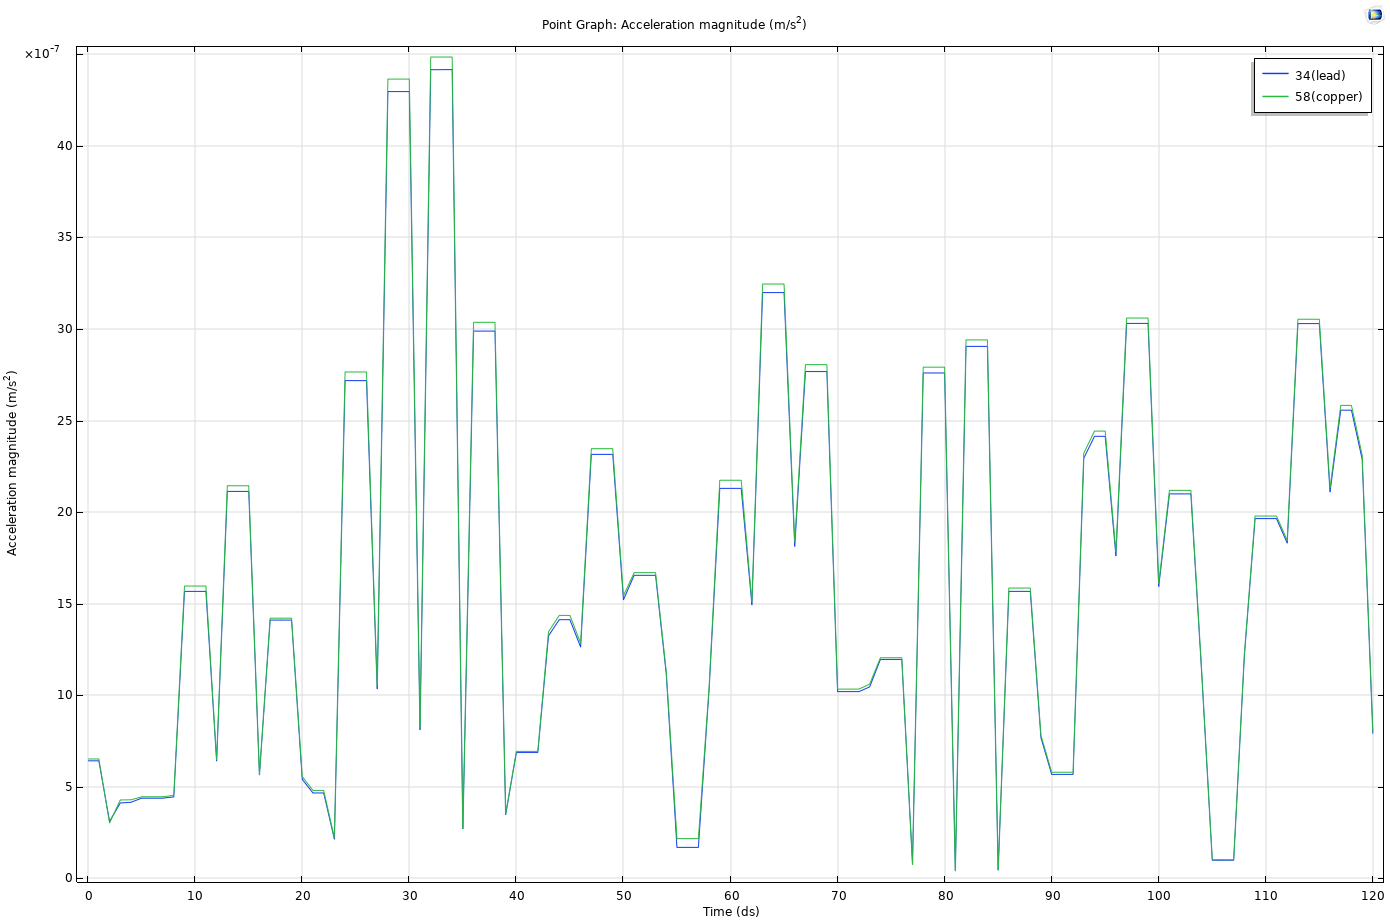
\includegraphics[width=0.4\hsize]{./Graph.png}
  \caption{The graph that distinguishes between lead and copper.}
  \label{fig:logo}
\end{figure}

% Uncomment for bibliography on each chapter.
% \bibliographystyle{plainnat}				
% \markright{\textit{Bibliography}}
% \renewcommand{\chaptername}{}
% \bibliography{my_references}

% \vfill


%%% Local Variables:
%%% mode: latex
%%% TeX-master: "DMSE-Thesis"
%%% End:
